\section{Performance comparison}
\label{sec:performance_comparison}

In this section, some of the new vehicle architectures are compared to the traditional vehicle to enlighten the different driving styles that lead to a faster or a slower lap. The track selected for the comparisons is Siena, described previously and shown in Figure~\ref{fig:siena_track}. Siena track presents low-speed curves in which dynamic camber control (DCC) architecture or four independent steering wheels (AS) impact substantially. The track is run clockwise from the start point, represented by the bold red line in Figure~\ref{fig:siena_track}. The thin red lines are spaced by a $\De\al=0.1$, and the black lines, also spaced by $\De\al=0.1$, are shifted from the red ones by $\al_s=0.05$. Additionally, the plot shows the enumeration of the turns, from 1 to 7, which will be useful for further observations.

First of all, a traditional vehicle (RWD FS) is compared with an AIWD FS vehicle, capable of applying four independent torques to the wheels. As already mentioned, this feature provides the highest improvement in performance. In the analyzed case, the vehicle is able to apply not only four driving torques, each one completely independent of the others, but also four independent braking torques. This is possible if we assume the vehicle has four separate oil lines or a different braking system. For this type of vehicle, usually driven by a human, this design is never applied due to the driver's inability to manage four control inputs, such as pedal forces. The decision to maintain the four independent braking torques is made here considering that the vehicles under study are not (yet) existing models and can be thought of as new architectures envisioned for future autonomous vehicle competitions. In this case, having more inputs would not be a problem unless some limits in the real-time computing power of the ECU are encountered --- a situation not discussed here. In this work, in fact, we focused on identifying and analyzing these solutions, which serve as a benchmark for maximizing vehicle performance, while intentionally postponing their implementation in a real vehicle to future designs.
%(Questa parte sotto e' poco chiara. Quello che facciamo noi fornisce un riferimento su come si dovrebbe guidare. E' chiaro che poi ti serve un controllore in feedback per fare tracking oppure per fare una pianificazione dinamica con re-planning tipo MPC che gestisce le discrepanze. Tuttavia questi sono aspetti che nella analisi corrente non sono considerati perche' andrebbero valutati in seconda battuta. Pero' non terrei il tono un po' negativo che traspare da questa parte di testo. Direi semplicemente che questi aspetti sarebbero da analizzare in 'future work' e per 'mettere a terra' una soluzione che noi analizziamo a livello funzionale e di potenzialita'.)
%In general, in worth bearing in mind that these solutions cannot be implemented ``as is'' for feed-forward control for multiple reasons. The most important is that the errors arising from the modeling process and discretization lead to a solution that is almost correct, and thus applying the resulting inputs would generate a different evolution of the system, resulting in a significant final cumulative error. Therefore, having a controller would be mandatory, and the high number of control channels would call for appropriate analyses. %The results of this case will justify the decision to separately compare RWD and AWD vehicles.

\begin{figure}[]
	\centering
	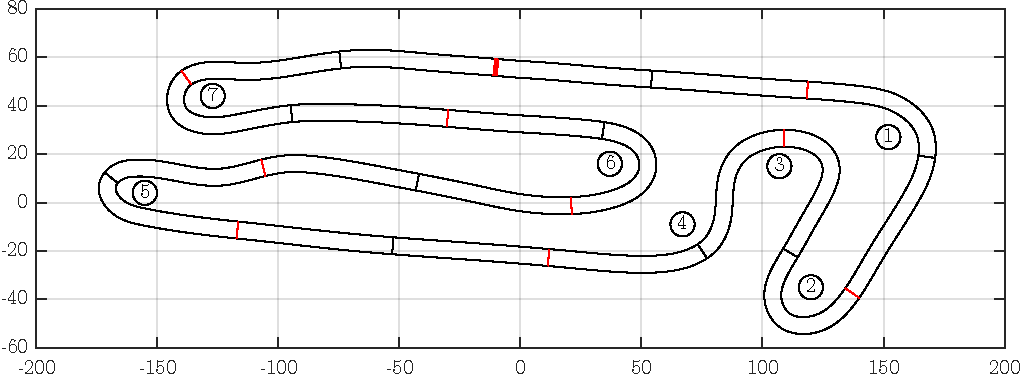
\includegraphics[scale = .85]{Images/DrivingStyles/siena_track.pdf}
	\caption{Siena Circuit. The bold red line indicates the starting point, while the other red lines are equally spaced by a $\De\al=0.1$. The black lines are also spaced like the red ones but are shifted by $\al_s=0.05$. The track is run in a clockwise direction. The curves, consisting of 2 to the left and 5 to the right, are sequentially numbered based on the order of encounter.}
	\label{fig:siena_track}
\end{figure}

\subsection{All Independent Wheel Drive, Forward Steering Vehicle - AIWD FS}
\label{sec:awdfs}
To perform a valid comparison between vehicles with different powertrain, they are assumed to have the same maximum (and maximum negative, i.e. braking) power. While the RWD vehicle, modeled with an open differential, will have identical torques on the driving wheels to generate power, the AIWD vehicle will  optimally distribute the power among four wheels, maintaining the same total value of the RWD vehicle.

For most turns, the two vehicles follow different trajectories, with the AIWD staying significantly closer to the inside boundary of the track during turns, as it can be observed in Figure~\ref{fig:rwdfs_awdfs_uayey}, third panel. See also the accompanying video~\cite{video:AWDFS:2024}.
The third plot, in fact, depicts the evolution of the variable $e_y (m)$, which represents the lateral distance, described in $\sref{S}$ components, of the CoM with respect to the center-line, at the corresponding $\al$. In a left turn, positive values of $e_y$ correspond to points that are closer to the inner boundary. Vice versa, in a right turn, negative values correspond to points that are closer to the inner boundary. Each of the three plots shown in Figure~\ref{fig:rwdfs_awdfs_uayey} includes green dash-dot lines marking the turns, while the forward speed plot (first panel) additionally displays the turn numbers, with labels placed over double-ended arrows. The enumeration follows the one described in Figure~\ref{fig:siena_track}, and each label indicates a letter that identifies the direction of the curve (L for left turns, R for right turns). Again from Figure~\ref{fig:rwdfs_awdfs_uayey}, third plot, we can observe that the AIWD vehicle begins to move toward the inner boundary of the track before the RWD vehicle. This behavior is evident in turn 2, which starts at $\al=0.2$, where the AIWD vehicle (blue line) reaches the inner boundary before the RWD (red line), with a difference of $\de\al=0.01$. On this track, this difference in curvilinear abscissa corresponds to 12.9\,m. Consequently, as the vehicles approach turn 2, the AIWD vehicle reaches the inner boundary approximately 13\,m ahead of the RWD vehicle, indicating a significantly different driving style.
%Di cosa stai parlando? dove devo guardare? a quale $\al$? non si segue...
%(quale e' la turn 2? cosa deve guardare il lettore? cosa sono le 1R, 2R, 3L sopra nel primo grafico? non sono mai state introdotte o spiegate)
\begin{figure}[h]
	\centering
	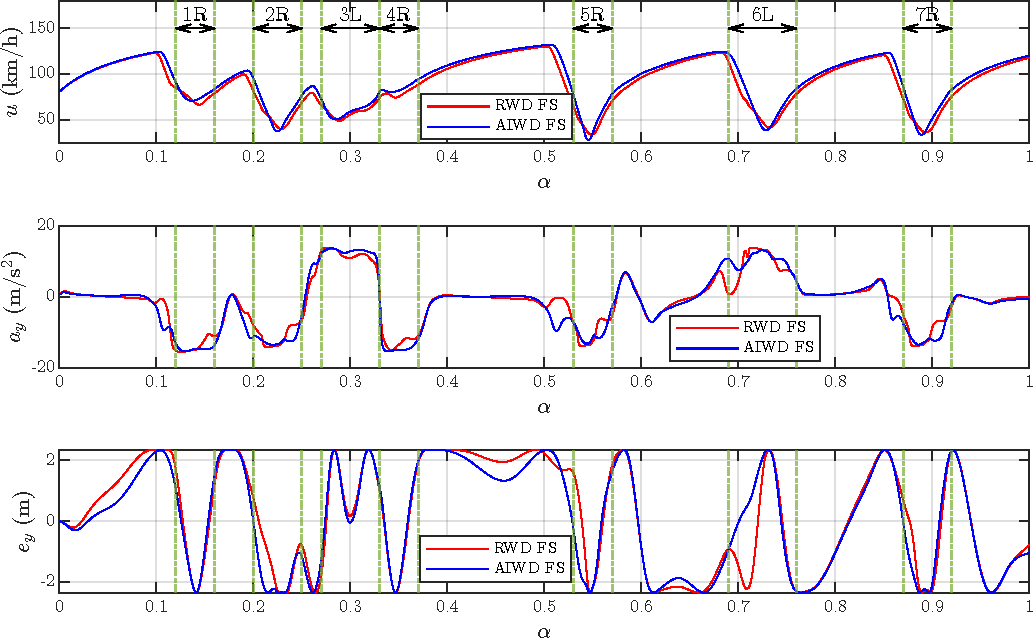
\includegraphics[scale = .8]{Images/DrivingStyles/rwdfsaiwdfs_p.pdf}
	\caption{
		Forward speed $u$, lateral acceleration in body components $a_y$ and $e_y$ evolution for RWD FS and AIWD FS vehicle, in red and blue respectively, over curvilinear abscissa $\al$. The quantity $e_y$ represents the lateral distance, in $\sref{S}$ reference, of the CoM with respect to the center-line at the corresponding $\al$.
		%Positive values in a left turn correspond to points that are closer to the inner limit, and vice versa in a right turn, positive values correspond to points that are closer to the outer limit.
		The turns are indicated in the forward speed plot (first panel) with the corresponding number (see Figure~\ref{fig:siena_track}) and a letter that identifies the direction (L for left turns and R for right turns). The more positive the values, the closer the trajectory to the left edge of the track, while the more negative the values, the closer the trajectory to the right edge.}
	\label{fig:rwdfs_awdfs_uayey}
\end{figure}

Still referring to Figure~\ref{fig:rwdfs_awdfs_uayey}, in particular to the first plot, which shows the forward speed $u$ over the curvilinear abscissa $\al$, we notice that, during cornering, the AIWD vehicle (blue line) approaches the point of minimum speed earlier than the RWD vehicle (red line).
The combination of this trend, and the previously analyzed tendency to remain closer to the inner boundary while cornering, allows the AIWD vehicle to exit with higher forward speed than the RWD vehicle. This affects positively the lap time.

In the second plot of Figure~\ref{fig:rwdfs_awdfs_uayey}, which reports the lateral acceleration $a_y$ over the curvilinear abscissa $\al$, we can notice that during cornering the AIWD vehicle (blue line) maintains a higher mean absolute value of the lateral acceleration.

In particular, traveling the chicane composed by turn 3 and 4, starting at $\al = 0.27$, the lateral acceleration $a_y$ of the AIWD FS vehicle (blue line) is greater (in magnitude) than the lateral acceleration of the RWD FS vehicle (red line), except for the small range, in which $\al\in[0.27, 0.28]$.

Still referring to the second plot of Figure~\ref{fig:rwdfs_awdfs_uayey}, and  focusing on turn 4, starting approximately at $\al = 0.33$, the lateral acceleration $a_y$ of the AIWD vehicle has smaller variation than the lateral acceleration of the RWD vehicle, maintaining almost a constant value during cornering, denoting a smoother behavior.
%This behavior can be explained by considering that having four driving torques allows the vehicle to achieve a higher absolute yaw moment, and hence a higher yaw rate $r$, which results in higher lateral acceleration $a_y$. In fact if we consider, for simplicity, a 2D vehicle model for handling, as the one described in~\cite[Chapter~3.2]{Guiggiani:book:2023}, with the hypothesis listed in the introduction of the chapter, is possible to express the lateral acceleration as follows:
%\begin{equation}\label{eq:ayguiggiani}
%a_y = \dot{v} + ur,
%\end{equation}
%where $u$, $v$ and $r$ are respectively, longitudinal and lateral velocity, and yaw rate.


%Apart from the different trajectory, the AWD vehicle pushes the wheels close to the grip limit not only in the lateral direction but also in the longitudinal direction, thereby generating greater tangential forces.

%Qui non si capisce dove vuoi arrivare. Il ragionamento (o la spiegazione associata) non e' chiaro. Hai richiamato la formula della $a_y$ per cosa? Cosa aumenta diminuisce nei due termini? Non si capisce, prova a rileggerti cercando di desumere il messaggio solo da cio' che e' scritto. %Considering this evidence, we can affirm that the two vehicles have significantly different driving styles, and thus the effects of the added features could be misinterpreted.

\subsection{Rear Wheel Drive, All Steering Vehicle - RWD AS}
We can observe in Figure \ref{fig:RWD_AS_toes}, first plot, the road wheel angles $\de_{i,j}$ of the four wheels with respect to the curvilinear abscissa $\al$ for the RWD AS vehicle. It is worth recalling that, during cornering, this vehicle can exhibit different road wheel angle values for the wheels of the same axle.

In the first plot, the color code is such that wheels of the same axle share the color (red for the front axle, blue for the rear axle), while wheels of the same side share the same line style (solid line for the left side, dashed line for the right side). In the second plot, the forward speed $u$ with respect to the curvilinear abscissa $\al$ is depicted.
In both plots, the green vertical lines mark the start and end point of the turns. In the lower plot, the turns are labeled with a progressive number, according to Figure~\ref{fig:siena_track} and a letter indicating its direction (L for left-hand turns and R for right-hand turns).

Although a slight penalization is applied to the cost function to avoid discordant wheel angles on the same axle during turns, the independent behavior of the wheels allows for better control of ground forces and their direction, enhancing turning performance. This is especially noticeable in turn 5 (right turn), where the left wheels steer more than the right, and in turn 6 (left turn), where the right wheels steer more than the left. See also the accompanying video~\cite{video:RWDAS:2024}. Generally, the outer wheel, which bears a greater vertical load due to lateral transfer, has a larger road wheel angle thus generating more lateral force, while the inner wheel steers less since it contributes less to the total lateral force.
%\begin{figure}[h]
%	\centering
%	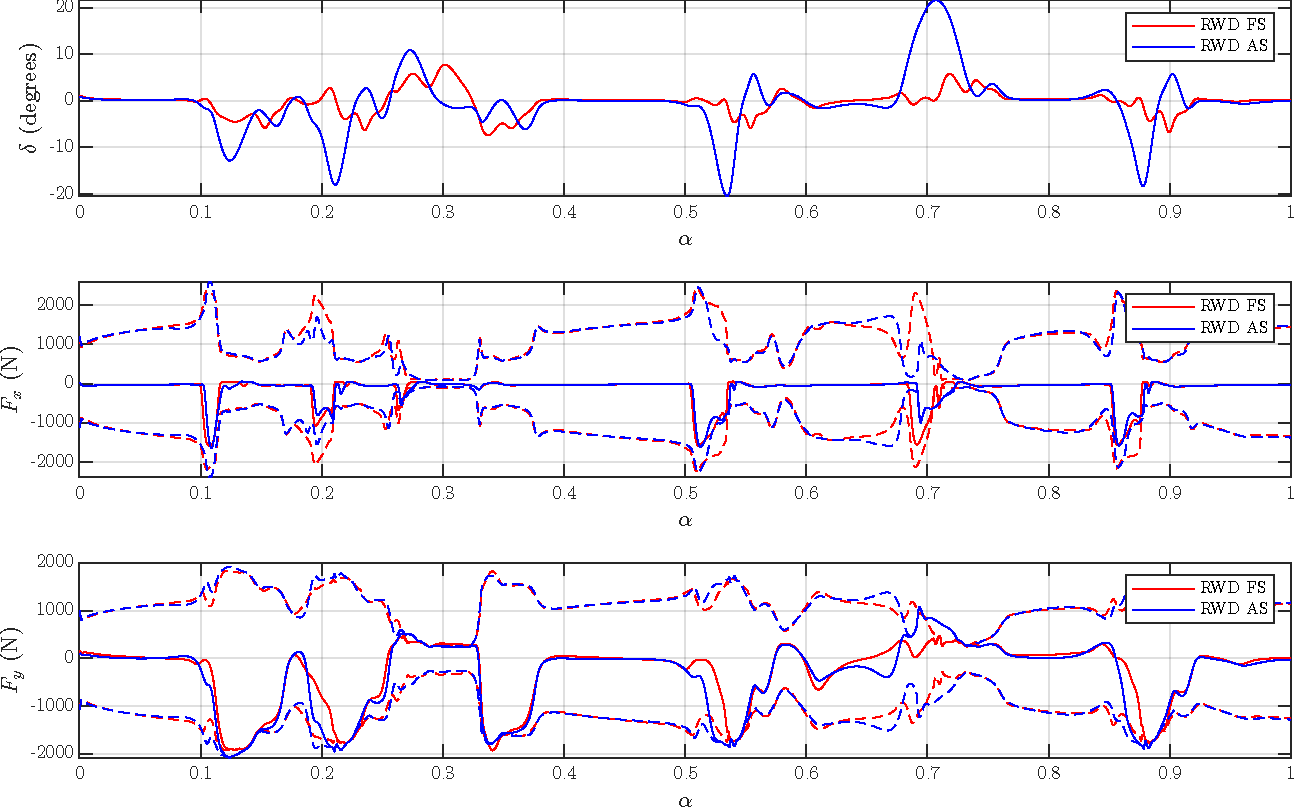
\includegraphics[scale = .65]{Images/DrivingStyles/rwdfs_rwdas_toeForces.pdf}
%	\caption{Toe angle $\de$, $F_x$ and $F_y$ forces for the front left wheel of a RWD FS and a RWD AS vehicle, in red and blue respectively. Dashed lines in the forces plots indicate the maximum and minimum force reachable.}
%	\label{fig:rwdfs_rwdas_toeForces}
%\end{figure}
\begin{figure}[h]
	\centering
	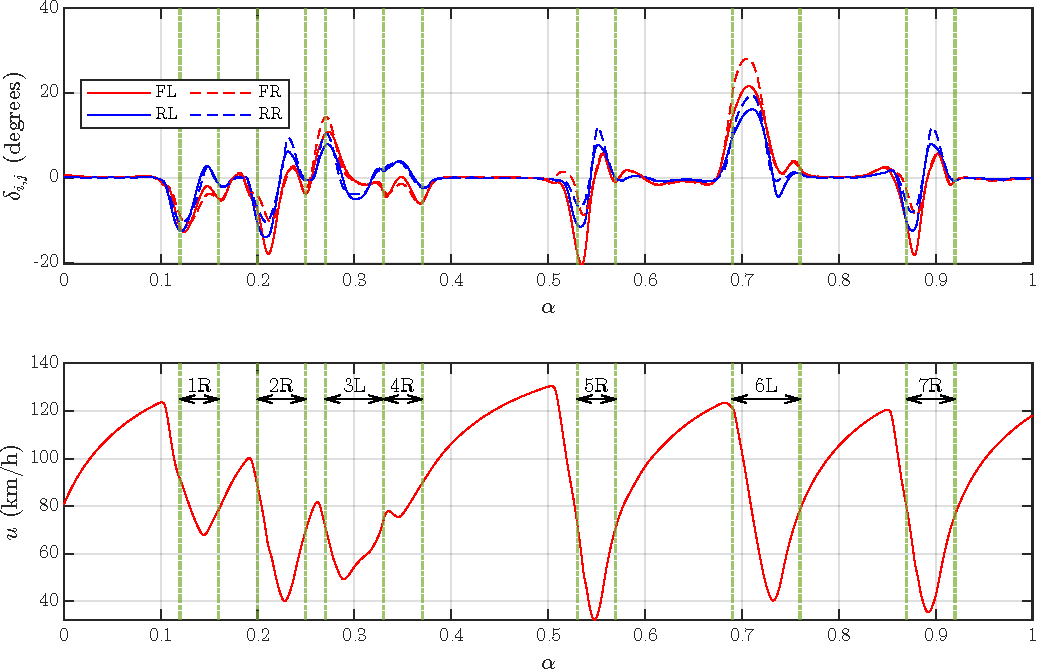
\includegraphics[scale = .8]{Images/DrivingStyles/RWD_AS_toes.pdf}
	\caption{Road wheel angle $\de$ of all wheels (above), and forward speed $u$ (below), evolution over curvilinear abscissa $\al$. As reported in the legend, wheels of the same axle share the same color, while wheels of the same side (left/right) share the same line style. The green dash-dot lines represent the starting and ending point of turns. The turns are indicated in the forward speed plot with the corresponding number (see Figure~\ref{fig:siena_track}) and a letter that identifies the direction (L for left turns and R for right turns).}
	\label{fig:RWD_AS_toes}
\end{figure}

Another aspect worth noting is the behavior of the rear wheels in relation to the front ones. In fact, the rear wheels steer in phase with the front wheels for most of the corners and for most of the corner entrances, except for some cases where, in the slower part of the turn, the rear wheels steer in counterphase with the front wheels.
In particular, referring again to Figure~\ref{fig:RWD_AS_toes}, it is possible to observe that in turn 2-5-7 the front and rear road wheel angles are concordant, while in the remaining turns (1-3-4-6), the road wheel angles are discordant for most part of the turn.
This behavior is generally consistent with Guiggiani's analysis of MAP's (Map of Achievable Performance) for a Single-Track model of vehicle. In fact, in~\cite[Section~6.8.1]{Guiggiani:book:2023} the author affirms that a desired behavior is to have a vehicle where the $\be$ angle spans a small range.
This can be achieved by having in-phase rear steering at high forward speeds and counter-phase rear steering at low forward speeds.

Although a general rule like this may not hold true for every corner on the track, it nonetheless represents the desired trend to optimize performance, which is here confirmed by quantitative lapsim outputs.
It also may be worthwhile to point out that a human driver can drive differently with respect to the optimizer, due to the fact that it lacks the perfect view of the track beforehand which, on the other hand, is profitably exploited by the optimizer.
%This in also confirmed if we observe that the amplitude of the beta angle, slightly reduced in many turns.
%\begin{figure}[h]
%	\centering
%	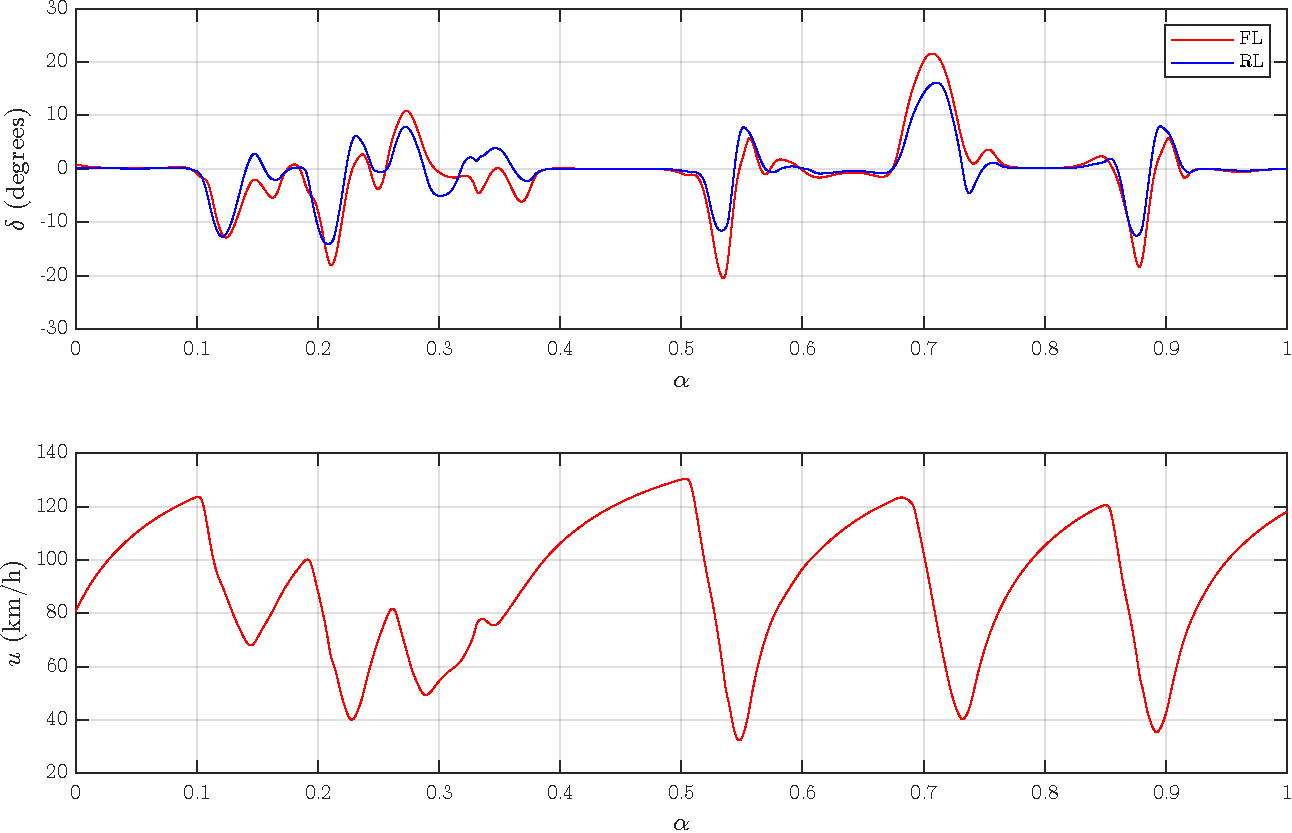
\includegraphics[scale = .65]{Images/DrivingStyles/rwdas_toe.pdf}
%	\caption{Toe angle $\de$ for the front and rear left wheel, and forward speed $u$ for a RWD AS vehicle. (For the toe angle, only the left side is plotted for clarity and readability, considering that the wheels on the same axle steer in-phase with each other)}
%	\label{fig:rwdas_toe}
%\end{figure}

%The last aspect we discuss here is the approach to the turns. The AS vehicle brakes less than the FS vehicle and approaches the corners with a higher forward speed. This behavior can be explained by considering that, with better control of the ground forces, the vehicle reaches the grip limit at higher velocities and lateral accelerations. Not only does the higher limit contribute to this, but having four steered wheels also generates a higher resistance force. This becomes clear when we decompose the four lateral forces of the wheels in the vehicle reference system.

\subsection{Rear Wheel Drive, Forward Steering, Dynamic Camber Control - RWD FS DCC}
The ability to adjust the camber of each wheel during cornering allows the vehicle to maximize the ground forces even more. In fact, in a traditional vehicle, the position and orientation of the wheels during a turn are determined by the passive motion of the suspension, in addition to the steering system for the front wheels. This means that, even if the suspension is well designed, the position of the wheels will not be always the best for performance and could be improved in each turn.

The first plot of Figure~\ref{fig:rwdfs_rwdfsdcc_gammaFyFR} shows the camber angles $\ga$ of the front right wheel (FR) over the curvilinear abscissa $\al$ for a RWD FS vehicle (red line) and for a RWD FS DCC vehicle (blue line), respectively.
The second plot of Figure~\ref{fig:rwdfs_rwdfsdcc_gammaFyFR} shows the lateral force $F_y$ of the front right wheel (FR) for the RWD FS vehicle (red solid line) and for the RWD FS DCC vehicle (blue solid line). Furthermore the maximum and minimum achievable lateral forces are shown in dashed lines and following the colors of the solid lines (RWD FS in red, RWD FS DCC in blue). Both plots show green dash-dot lines to delimit turns, while the first plot, in addition, reports labels with turn numbers (that follow the enumeration of Figure~\ref{fig:siena_track}), and an indication of the turn direction (L for left turns, R for right turns).

It is possible to note that, during cornering, e.g. turn 3, the camber tends to settle around a value of $-7.5$~degrees which contributes to increasing the lateral force by 128 N. This corresponds to a 7.6\% increase w.r.t. the baseline, which can be considered a significant achievement (see the zoomed area in the second plot at turn 3, where $\al\in [0.26, 0.33]$). See also the accompanying video~\cite{video:RWDFSDCC:2024}.

Similarly, in turn 6, starting at $\al = 0.69$, it can be observed that the maximum lateral force $F_y$ achievable is higher for the RWD FS DCC vehicle, implying a better wheel positioning relative to the road.
We remind that, according to the convention of positive lateral forces $F_y$ pointing to the left of the vehicle, ``the higher (more positive) the better'' is valid if we analyze a left turn, such as turn 3 or 6. Otherwise, in a right turn, an improvement on force limits would correspond to a lower minimum for achievable lateral force.
For this reason, considering here the front right (FR) wheel, we focus only on left turns.
%In the Figure \ref{fig:rwdfs_rwdfsdcc_gammaFyFR}, showing the camber angle $\ga$ evolution (above) and the lateral force $F_y$ (below) of the front right wheel over the curvilinear abscissa $\al$, the limits, indicated by dashed lines and coded with the same color of the actual forces, are higher than those of the traditional vehicle, implying a better wheel positioning relative to the road. This is more evident in the left turns, in which this wheel has a higher vertical load.

\begin{figure}[h]
	\centering
	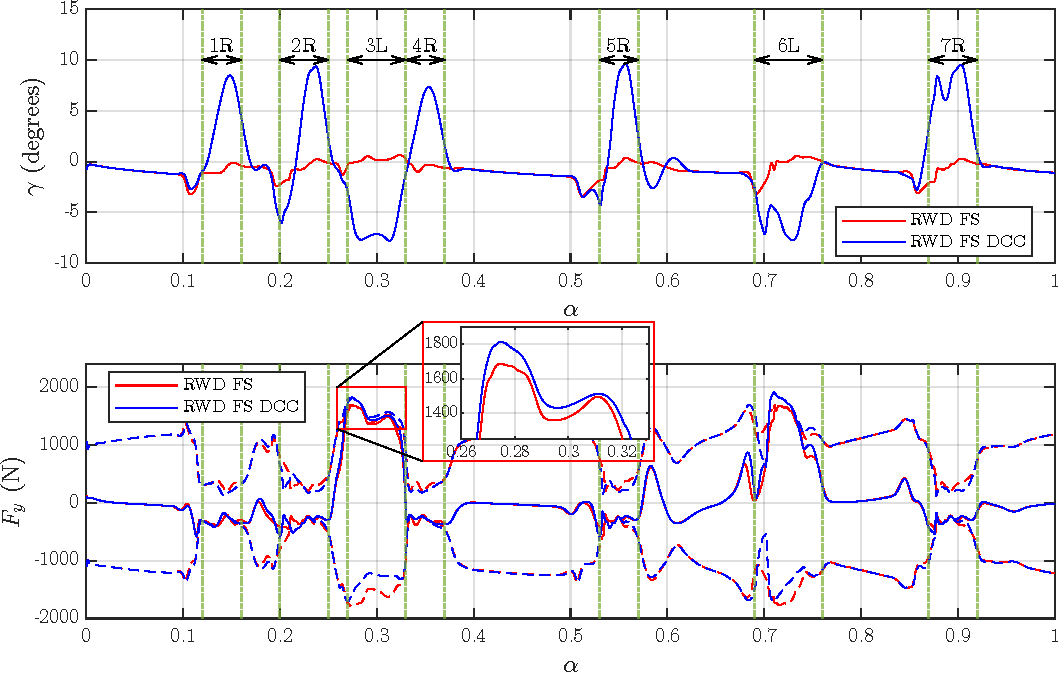
\includegraphics[scale = .8]{Images/DrivingStyles/rwdfs_rwdfsdcc_gammaFyFR.pdf}
	\caption{Camber angle $\ga$ (first plot), and lateral force $F_y$ (second plot) over curvilinear abscissa $\al$, for the front right wheel (FR) of a RWD FS (red line) and a RWD FS DCC (blue line) vehicle. The dashed lines represent the upper and lower limit of the forces for each vehicle, coded by the same color. The green dash-dot lines represent the starting and ending point of turns. The turns are indicated in the forward speed plot with the number and the letter that identifies the direction (L for left turns and R for right turns). The zoomed area reports the section with $\al\in [0.26, 0.33]$ to highlight the improvement of $\simeq 130$\,N in the lateral force achievable by Dynamic Camber Control (DCC).}
	\label{fig:rwdfs_rwdfsdcc_gammaFyFR}
\end{figure}

%The vertical loads from the optimization, combined with the tyre model, are used to analyze the behavior of the camber angle during cornering. In particular, the goal is to verify that the value assumed by the camber angle guarantees the maximum lateral force. In Figure~\ref{fig:dcc_lateralforce_gammaspan}, a zoomed-view of the lateral force $F_y$ of the front right wheel (FR) in first part of the turn 3 ($\al\in[0.268, 0.286]$) over the curvilinear abscissa $\al$ is presented. The solid curve in black represents the optimal lateral force derived from the optimization, obtained with a value of the camber angle $\gamma^*(\al)$, varying with the curvilinear abscissa. The dashed red curve represents the potential force obtained with the minimum value of the added camber $q_{hk,\text{max}}=9$~degrees (see Section~\ref{sec:cambersystemmodeling}). The other colored lines represent the lateral forces obtained with the same vertical load $F_z(\al)$ derived by the optimization, and varying the total camber angle $\ga\in[\ga^*(\al)-\De\ga,\ga^*(\al)+\De\ga]$, with $\De\ga = 4$ degrees. As we can observe, by varying $\ga$ such that $\ga = \ga^*(\al) + \de\ga$, with the value of $\de\ga$ coded by colors in the bar on the right side, the lateral force presents a peak that, especially in the second part of the plot, doesn't correspond to $\de$ equal to the limit value $\pm\De\ga$. After the first part of the curve, which presents a delay due to the fact that we command the second derivative of $q_{hk}$, the solution, adjusting the additional camber, coasts the maximum value of the force.

%\begin{figure}[h]
%	\centering
%	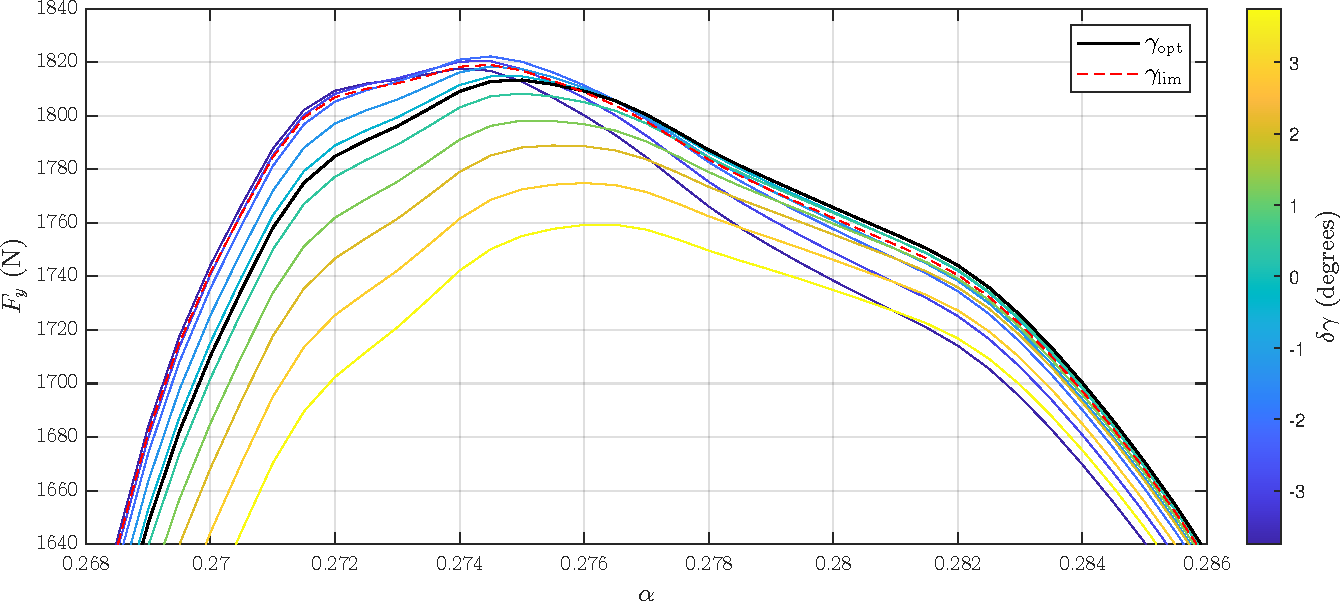
\includegraphics[scale = .65]{Images/DrivingStyles/dcc_lateralforce_gammaspan}
%	\caption{Reachable lateral forces $F_y$ over curvilinear abscissa $\al$ when spanning the camber angle $\ga\in[\ga^*(\al)-\De\ga,\ga^*(\al)+\De\ga]$, equivalent to a window of $\pm 4$ degrees centered on the optimal value $\ga^*(\al)$, which varies with curvilinear abscissa $\al$. The black line indicates the optimal value of the force, while the red dashed line indicates the force obtained with the maximum, or minimum, depending on the sign, value of the additional camber $\De\ga$. The colored lines represents level curves with constant $\De\ga$, but, in general, different $\ga$.}
%	\label{fig:dcc_lateralforce_gammaspan}
%\end{figure}

For brevity, we only mention that the RWD AS DCC vehicle combines the advantages of the previous two, thereby guaranteeing the highest performance. Similarly to the RWD AS vehicle, it steers more with the outer wheels thus exploiting the lateral load transfers; at the same time, as registered for the RWD FS DCC vehicle, it adjusts the camber during cornering to settle around the value of maximum ground force available.


%In Figure~\ref{fig:rwdfs_rwdasdcc}, upper plot, the evolution of the road wheel angles $\de_{i,j}$ with respect to the curvilinear abscissa $\al$ is depicted using the same conventions of Figure~\ref{fig:RWD_AS_toes}.
%The lower plot shows the lateral force $F_y$ evolution over the curvilinear abscissa $\al$ and the force bounds, with the same layout of Figure~\ref{fig:rwdfs_rwdfsdcc_gammaFyFR}, for a RWD FS and RWD AS DCC vehicle, depicted in red and blue, respectively.
%
%With reference to the upper plot, we can observe the behavior noted for the RWD AS vehicle, which steers more with the outer wheels thus exploiting the lateral load transfers.
%Similarly to the RWD FS DCC, this vehicle adjusts the camber during cornering to settle around the value of maximum ground force available. Still referring to turn 3, as done in the zoomed area of Figure~\ref{fig:rwdfs_rwdfsdcc_gammaFyFR}, the maximum increase of the force grows now up to 12.1\%. These two effects combined also allow the vehicle to navigate corners with higher driving torque on the rear wheels or, in general, less braking torque on all four wheels, thus resulting in a higher forward speed.
%\begin{figure}[h]
%	\centering
%	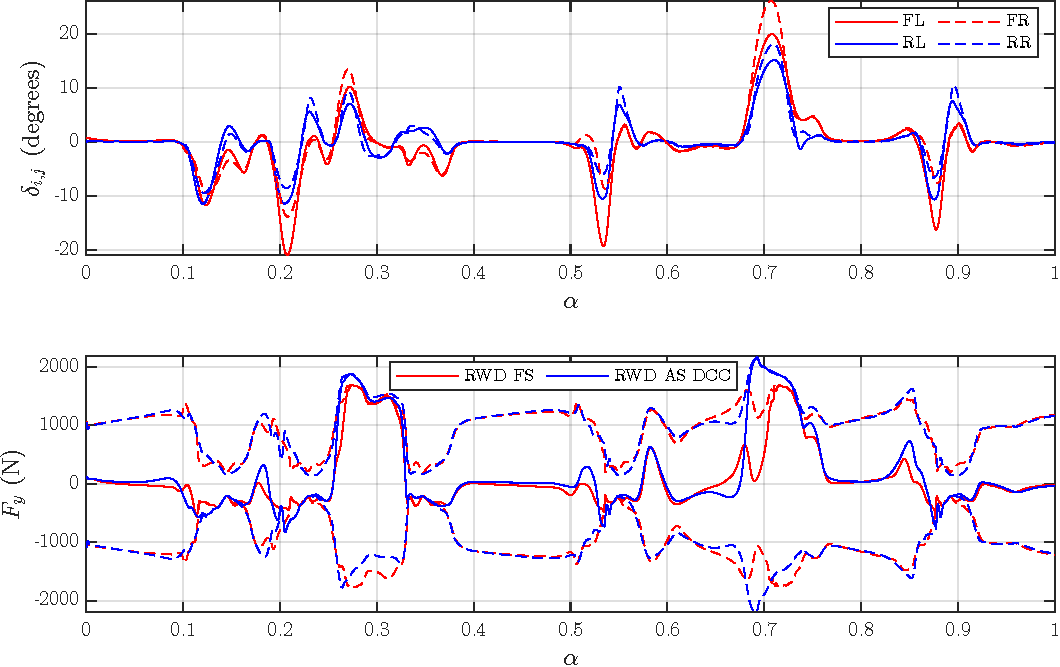
\includegraphics[scale = .8]{Images/DrivingStyles/rwdfs_rwdasdcc.pdf}
%	\caption{Road wheel angles $\de_{i,j}$ of all wheels of a RWD AS DCC vehicle over curvilinear abscissa $\al$ (upper plot), and lateral force $F_y$ over curvilinear abscissa $\al$ (lower plot), for the front right wheel (FR) of a RWD FS (red line) and a RWD AS DCC (blue line) vehicle. The dashed lines represent the upper and lower limit of the forces for each vehicle, coded by the same color.}
%	\label{fig:rwdfs_rwdasdcc}
%\end{figure}

\section{AIWD 0S DCC: in depth analysis}
This section aims to showcase that on a track with characteristics like the N\"{u}rburgring section used or Siena, whose results we present here, a vehicle able of applying four independent acceleration torques (AIWD) and dynamically controlling the camber (DCC) has a very significant advantage in terms of lap time and cornering performance.

To stress the power of these features, a vehicle with such characteristics but \emph{without steering abilities} (0S, zero steering) has been considered. See also the accompanying video~\cite{video:AWDOSDCC:2024}.
Cornering is still possible if the vehicles applies different torques to the wheels on the same axle, as we can observe in Figure~\ref{fig:awd0sdcc_deltaT}.
Here, the evolution of the torques applied to the wheels $T_{i,j}$ over the curvilinear abscissa $\al$ for the front axle (upper plot) and the rear axle (lower plot) is illustrated.
The left wheels (FL and RL) are plotted with red lines, while the right wheels (FR and RR) are plotted with blue lines. Similarly to the previous figures, the green dash-dot lines in both plots delimit the turns, while the labels in the first plot denote the turn number, according to Figure~\ref{fig:siena_track}, and a letter which discriminates the direction (L for left-hand turns, R for right-hand turns).

During turns 2-5-6-7, the torque of the inner wheel settles to zero, as is possible to observe in the first panel of Figure~\ref{fig:awd0sdcc_deltaT}. Here, the inner wheel starts a free rolling motion, with no applied torque by the motor.

Otherwise a different behavior emerges in turn 4, starting around $\al=0.33$. Here, the two wheels experience torques that are approximately mirror-symmetric with respect to the horizontal line $T=100$\,Nm, with the inner torque (FR, blue line) that assumes negative values closely to $\al=0.33$, without losing contact to the ground.
\begin{figure}[h]
	\centering
	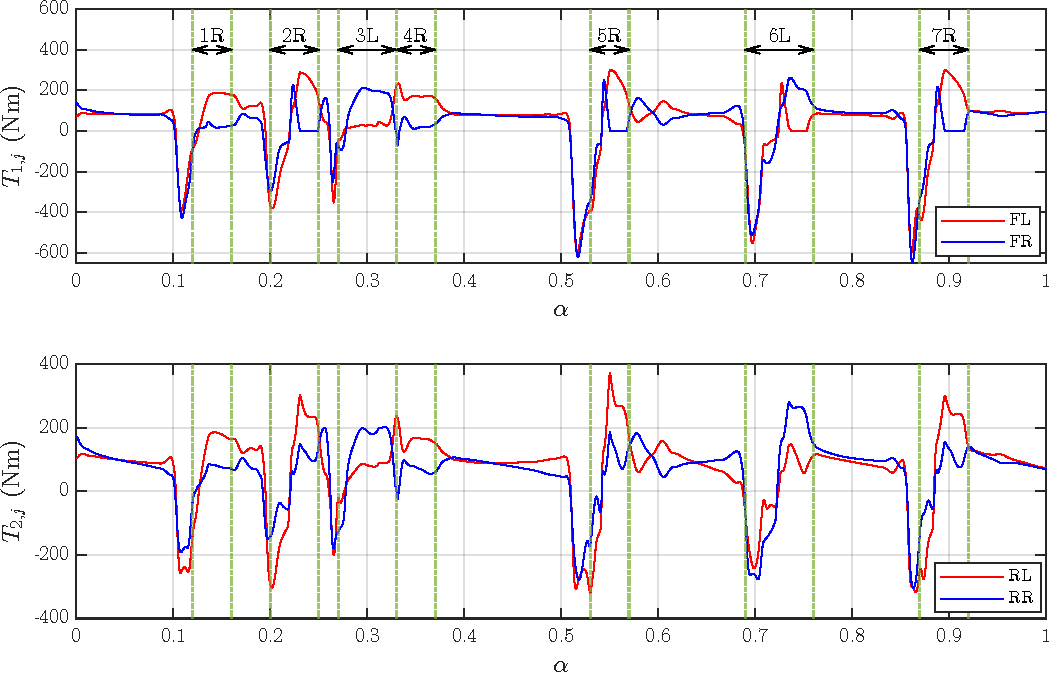
\includegraphics[scale = .8]{Images/DrivingStyles/awd0sdcc_deltaT.pdf}
	\caption{Wheel torques $T_{i,j}$ evolution over curvilinear abscissa $\al$, for the front wheels (above) and for the rear wheels (below) of a AIWD 0S DCC vehicle (0S indicates incapability of steering). The red lines refer to the left side while the blue lines refer to the right side. As for the previous plots, the green dash-dot lines indicates the turns, labeled in the first plot by the number and a letter L, for left turns, or R, for right turns.}
	\label{fig:awd0sdcc_deltaT}
\end{figure}

While the AIWD FS DCC vehicle completes a lap in 51.40 seconds, the AIWD 0S DCC vehicle does so in 51.64 seconds -- only 0.24 seconds slower but 3.66 seconds faster than a traditional RWD FS vehicle. This is achieved by properly adjusting camber and applying four independent torques, thus compensating for the lack of steering. The torque vectoring logic, used in both AIWD FS DCC and AIWD 0S DCC, plays a key role in optimizing turning maneuvers. By simply adjusting the intervention to avoid steering, the lap is completed with a 0.47\% increase in lap time compared to the AIWD FS DCC.
It is worth mentioning in passing that the model implements power limits as total values, neglecting potential motor saturation, and may lead to an overestimation of performance.
Therefore, this analysis should not be taken as a direct guideline for designing a AIWD 0S DCC vehicle but an informative case study highlighting factors relevant to cornering and steering.

%While an AWD FS DCC vehicle completes a lap in 51.40\,s, this vehicle (here named AWD 0S DCC) completes a lap in 51.64\,s, thus with only 0.24\,s more, but with 3.66\,s less than a traditional vehicle (RWD FS). This is possible because having the ability of adjust the camber and apply 4 independent torques compensate for the lack of steering. In particular the torque vectoring logic, used also for AWD FS DCC, provide the most for the turning maneuver, and hence, simply adjusting this intervention to avoid steering the vehicle completes the lap without significant problems. It's important to underline that, in the model, the power limits are implemented as total values, hence neglecting potential saturation of power for individual motors. This approach has been employed to compare different traction configurations (RWD/AWD); however, it may lead to an overestimation of achievable conditions. Nonetheless, this analysis should not be used as a guideline for designing a real AWD 0S DCC vehicle but rather serves as an informative case study that highlights various factors during cornering, including those related to steering. 